%%%%%%%%%%%%%%%%%%%%%%%%%%%%%%%%%%%%%%%%%%%%%%%%%%%%%%%%%%%%%%%%%%%%%%%%
%%%%%%%%%%%%%%%%%%%%%%%%%%%%%%%%%%%%%%%%%%%%%%%%%%%%%%%%%%%%%%%%%%%%%%%%
\begin{frame}
  \frametitle{Plan}

  \begin{itemize}
  \item 8 avril 2021 : \myhref{https://www.canal-u.tv/video/groupe_calcul/pourquoi_julia.60773}{Café Calcul - Pourquoi Julia ?} (F. Févotte)\\
     le problème des deux languages (script polyvalent + bas niveau performant)\\ $\Rightarrow$ \textcolor{violet}{\bf Julia}
  \item le problème du modèle de programmation (polyvalent, multi architecture)\\ $\Rightarrow$ \textcolor{violet}{\bf portabilité de performance}
  \end{itemize}

  \begin{center}
    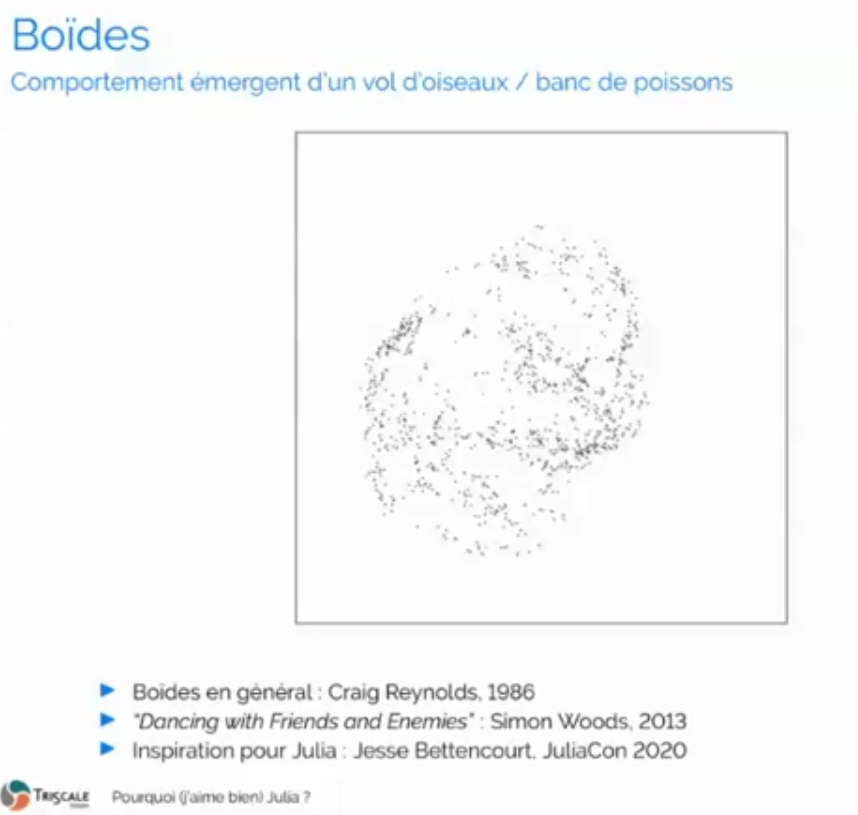
\includegraphics[width=3.5cm]{julia/pourquoi_julia1}
    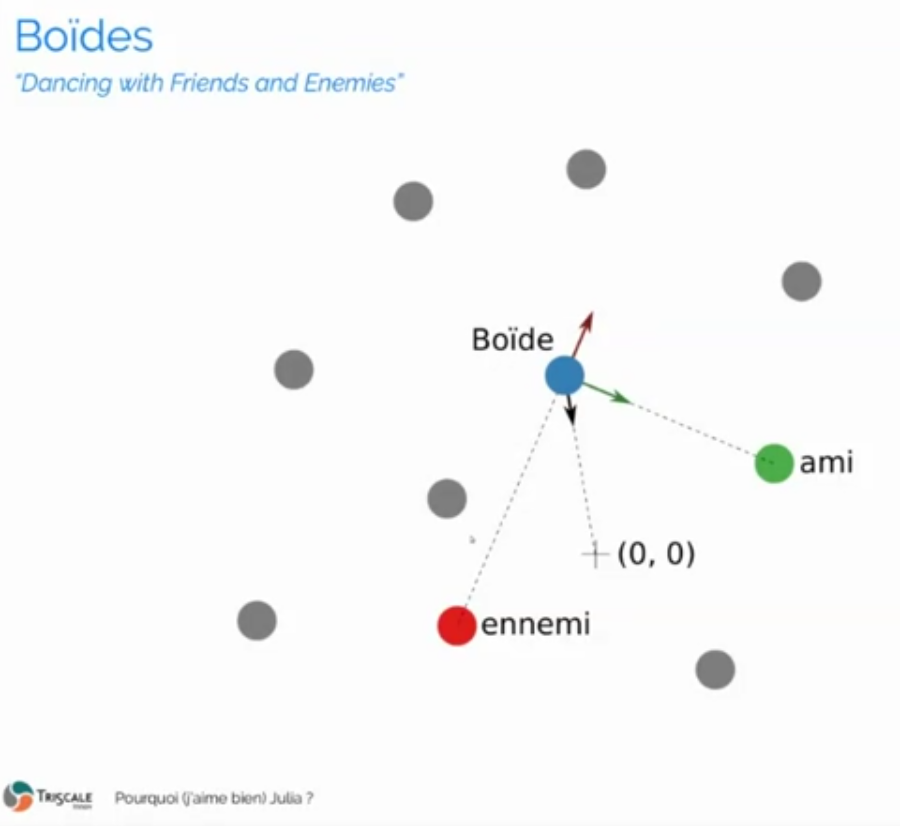
\includegraphics[width=3.5cm]{julia/pourquoi_julia2}
  \end{center}
  {\small nanoApp : (naively) revisiting boids flight with Kokkos, \myurl{https://github.com/pkestene/kboids}}

\end{frame}
